\documentclass{article}
\usepackage{../../Self_Style}

\title{Phys 115B HW 3}
\author{Zih-Yu Hsieh}
\date{\today}

\begin{document}
\maketitle

\section*{1 ND}
\begin{ques}\label{q1}
Hydrogen-like (variation on 4.19, or 4.16 in second edition [or 4.17 in the first edition])

Energy levels and eigenfunctions of a “hydrogenic” system can be obtained from those of the hydrogen atom by appropriately scaling mass and charge. Tritium ($^3$H) and $^3$He$^+$ are examples, which are linked by the process of beta decay, whereby a neutron in the tritium nucleus can convert to a proton by emitting a neutrino and an energetic electron which escapes the resulting $^3$He$^+$ ion.
\begin{itemize}
\item[(a)] For a 1-electron atom with a nucleus of charge $Ze$, find an expression for the Bohr radius and the Bohr energies as appropriate multiples of the hydrogen values

\item[(b)] Find the Bohr radius of tritium (you can approximate $m_e/m_p$ as zero)

\item[(c)] Find the Bohr radius of $^3$He$^+$

\item[(d)] A tritium atom is in its ground state. It undergoes a beta decay, which turns the tritium nucleus into a $^3$He nucleus. Assume that the decay is instantaneous and that it does not disturb the wavefunction of the bound electron. Calculate the probability that the electron will be found in the ground state of $^3$He$^+$

\item[(e)] The emitted electron leaves with an energy of about 6 keV. The recoil from this emission gives a kick to the $^3$He nucleus (Newton’s second law and all that). Find the energy and velocity of the $^3$He recoil, and determine whether we were correct to ignore this effect in the previous part.
\end{itemize}
\end{ques}

\begin{proof}
    
\end{proof}

\newpage

\section*{2 D}
\begin{ques}\label{q2}
Commutators

\begin{itemize}
\item[(a)] Work out the commutators $[L_z, x]$, $[L_z, p_x]$, $[L_z, y]$, $[L_z, p_y]$, $[L_z, z]$, $[L_z, p_z]$.

\item[(b)] Use those results to verify that $[L_z, L_x] = i\hbar L_y$

\item[(c)] Find the commutators $[L_z, r^2]$ and $[L_z, p^2]$.

\item[(d)] Show that a Hamiltonian with a spherically symmetric potential $V(r) = V(r)$ commutes with all components of $\bL$, and that $H$, $L^2$, and $L_z$ are compatible observables.
\end{itemize}
\end{ques}

\begin{proof}
    First, recall the definitions of each angular momentum operators:
    \begin{align}
        L_x &=yp_z-zp_y,\quad L_y=zp_x-xp_z,\quad L_z=xp_y-yp_x
    \end{align}
    Also, recall the commutation relations of position and momentum operators:
    \begin{align}
        u,v\in \{x,y,z\},\quad [u,p_v]=i\hbar \delta_{uv},\quad [u,v]=0,\quad [p_u,p_v]=0
    \end{align}
    \begin{itemize}
        \item[(a)] The desired commutators are as follow:
        \begin{align}
            [L_z,x] &= (xp_y-yp_x)x - x(xp_y-yp_x) \\
            &= x^2p_y - y(xp_x - i\hbar)-x^2p_y + xy p_x\\
            &= i\hbar y
        \end{align}
        \begin{align}
            [L_z,p_x] &= (xp_y-yp_x)p_x - p_x(xp_y-yp_x)\\
            &= xp_yp_x - y(p_x)^2 - (x p_x-i\hbar)p_y + y (p_x)^2\\
            &= i\hbar p_y
        \end{align}
        \begin{align}
            [L_z,y] &= (xp_y-yp_x)y-y(xp_y-yp_x)\\
            &= x(yp_y - i\hbar) - y^2p_x - yxp_y + y^2p_x\\
            &= -i\hbar x
        \end{align}
        \begin{align}
            [L_z,p_y] &= (xp_y-yp_x)p_y - p_y(xp_y-yp_x)\\
            &= x(p_y)^2 - yp_xp_y - x(p_y)^2 + (yp_y - i\hbar)p_x\\
            &= -i\hbar p_x
        \end{align}
        \begin{align}
            [L_z,z] &= (xp_y-yp_x)z-z(xp_y-yp_x) = 0
        \end{align}
        \begin{align}
            [L_z,p_z] &= (xp_y-yp_x)p_z-p_z(xp_y-yp_x)=0
        \end{align}

        \hfil

        \item[(b)] Using the commutation relation from part (a), we have:
        \begin{align}
            [L_z,L_x] &= L_z(yp_z-zp_y)-(yp_z-zp_y)L_z\\
            &= (yL_z - i\hbar x)p_z - zL_z p_y - (yp_z-zp_y)L_z\\
            &= yp_zL_z - i\hbar xp_z - z(p_yL_z - i\hbar p_x) - (yp_z-zp_y)L_z\\
            &= i\hbar (zp_x - xp_z) = i\hbar L_y
        \end{align}

        \hfil

        \item[(c)] Again, using the commutation relations in (a), we have:
        \begin{align}
            [L_z,r^2] &= [L_z,x^2]+[L_z,y^2]+[L_z,z^2]\\
            &= (L_zx)x - x(xL_z)+(L_zy)y-y(yL_z)\\
            &= (L_zx)x - (xL_z)x + x(L_zx)-x(xL_z)+(L_zy)y-(yL_z)y+y(L_zy)-y(yL_z)\\
            &= [L_z,x]x + x[L_z,x]+[L_z,y]y+y[L_z,y]\\
            &= i\hbar yx + x\cdot i\hbar y -i\hbar x y + y \cdot (-i\hbar x)\\
            &= 0
        \end{align}
        \begin{align}
            [L_z,p^2] &= [L_z,p_x^2]+[L_z,p_y^2]+[L_z,p_z^2]\\
            &= (L_zp_x)p_x-p_x(p_xL_z)+(L_zp_y)p_y-p_y(p_yL_z)\\
            &= (L_zp_x)p_x-(p_x L_z)p_x+p_x(L_zp_x) - p_x(p_xL_z)+(L_zp_y)p_y-(p_yL_z)p_y + p_y(L_zp_y)-p_y(p_yL_z)\\
            &= [L_z,p_x]p_x + p_x[L_z,p_x]+[L_z,p_y]p_y+p_y[L_z,p_y]\\
            &= i\hbar p_yp_x + p_x\cdot i\hbar p_y -i\hbar p_x p_y + p_y \cdot (-i\hbar p_x)\\
            &= 0
        \end{align}

        \hfil

        \item[(d)] Consider a Hamiltonian with spherically symmetric potential $H = \frac{p^2}{2m}+V(r)$, first it's clear that from part (c), one has $[L_z,p^2]=0$. After changing the coordinates (i.e. swapping order of $x,y,z$), using the spatial symmetry one can also claim that $[L_u,p^2]=0$ for all $u\in\{x,y,z\}$.
        
        So, to prove each component of $\bL$ commutes with $H$, it suffices to consider for the spherically symmetric potential $V(r)$.

        Given the definition $r=\sqrt{x^2+y^2+z^2}$, one has $\frac{\partial f}{\partial u} = \frac{\partial r}{\partial u}\frac{\partial f}{\partial r} = \frac{u}{\sqrt{x^2+y^2+z^2}}\frac{\partial f}{\partial r} = \frac{u}{r}\frac{\partial f}{\partial r}$ for any differentiable function $f$. Therefore, we have:
        \begin{align}
            [L_z,V(r)] &= (xp_y-yp_x)V(r) - V(r)(xp_y-yp_x)\\
            &= -i\hbar \left(x\frac{\partial}{\partial y}-y\frac{\partial}{\partial x}\right)V(r) - V(r)(xp_y-yp_x)\\
            &= -i\hbar\left(x\left(\frac{y}{r}\frac{\partial V}{\partial r} + V(r)\frac{\partial}{\partial y}-y\left(\frac{x}{r}\frac{\partial V}{\partial r}+V(r)\frac{\partial}{\partial x}\right)\right)\right)- V(r)(xp_y-yp_x)\\
            &= -i\hbar \cdot V(r)(x\frac{\partial}{\partial y}-y\frac{\partial}{\partial x})-V(r)(xp_y-yp_x)\\
            &= V(r)(xp_y-yp_x)-V(r)(xp_y-yp_x)=0
        \end{align}
        Hence, this shows that $L_z$ commutes with $V(r)$ as operator. Since $L_z$ commutes with all the components of the Hamiltonian $H$, one can say $[L_z,H]=0$. By the same spatial symmetry argument, one can also show that $[L_u,H]=0$ for all $u\in\{x,y,z\}$. This concludes that all components of $\bL$ commutes with $H$.

        Finally, since $L^2 = L_x^2+L_y^2+L_z^2$, it's clear that all of its components commute with $H$ (when $H$ is endowed with a spherically symmetric potential). Also, from the calculation before it's clear that $L_z$ commutes with $H$, and $L^2$ commutes with $L_z$. Therefore, $H,L^2,L_z$ are compatible observables.
    \end{itemize}
\end{proof}

\newpage

\section*{3 ND}
\begin{ques}\label{q3}
Normalizing $L_+$ and $L_-$ (Griffiths 4.21, 4.18 in second edition)

The raising and lowering operators change the value of $m$ by one unit:
$$L_+ f_\ell^m = (A_\ell^m)f_\ell^{m+1},\quad L_- f_\ell^m = (B_\ell^m)f_\ell^{m-1}$$
where $A_\ell^m$ and $B_\ell^m$ are constants. 

\emph{Questions:} What \emph{are} they, if the eigenfunctions are to be normalized?

\emph{Hint:} First show that $L_\mp$ is the hermitian conjugate of $L_\pm$ (since $L_x$ and $L_y$ are observables, you may assume they are hermition...but prove it if you like); then use the following equation:
$$$$
\emph{Answer:}
$$A_\ell^m = \hbar\sqrt{\ell(\ell+1)-m(m+1)} = \hbar\sqrt{(\ell-m)(\ell+m+1)}$$
$$B_\ell^m = \hbar\sqrt{\ell(\ell+1)-m(m-1)}=\hbar\sqrt{(\ell+m)(\ell-m+1)}$$
Note what happens at the top and bottom of the ladder (i.e. when you apply $L_+$ to $f_\ell^\ell$ or $L_-$ to $f_\ell^{-\ell}$)
\end{ques}

\begin{proof}
    
\end{proof}

\newpage

\section*{4 ND}
\begin{ques}\label{q4}
Rigid Rotor (Griffiths 4.27 a, b, c only, 4.24 in the second edition)

Two particles (masses $m_1$ and $m_2$) are attached to the ends of a massless rigid rod of length $a$. The system is free to rotate in three dimensions about the (fixed) center of mass.
\begin{itemize}
    \item[(a)] Show that the allowed energies of this \textbf{rigid rotor} are 
    $$E_n = \frac{\hbar^2}{2I}n(n+1)\quad (n=0,1,2,...),\quad\quad I:=\frac{m_1m_2}{m_1+m_2}a^2$$
    is the moment of inertia of the system. 

    \emph{Hint:} First express the (classical) energy in terms of the angular momentum.

    \item[(b)] What are the normalized eigenfunctions for this system? (Let $\theta$ and $\phi$ define the orientation of the rotor axis.) What is the degeneracy of the $n$th energy level?
    
    \item[(c)] What spectrum would you expect for this system? (Give a formula for the frequencies of the spectral lines.)
    
    \emph{Answer:} $\nu_j = \frac{\hbar j}{2\pi I}$, $j=1,2,3,...$.

    \item[(d)] Figure 4.13 shows a portion of the rotational spectrum of carbon monoxide (CO). What is the frequency separation ($\Delta \nu$) between adacent lines? Look up the masses of $^12 C$ and $^16 O$, and from $_1,m_2$, and $\Delta \nu$ determine the distance between the atoms.
    
    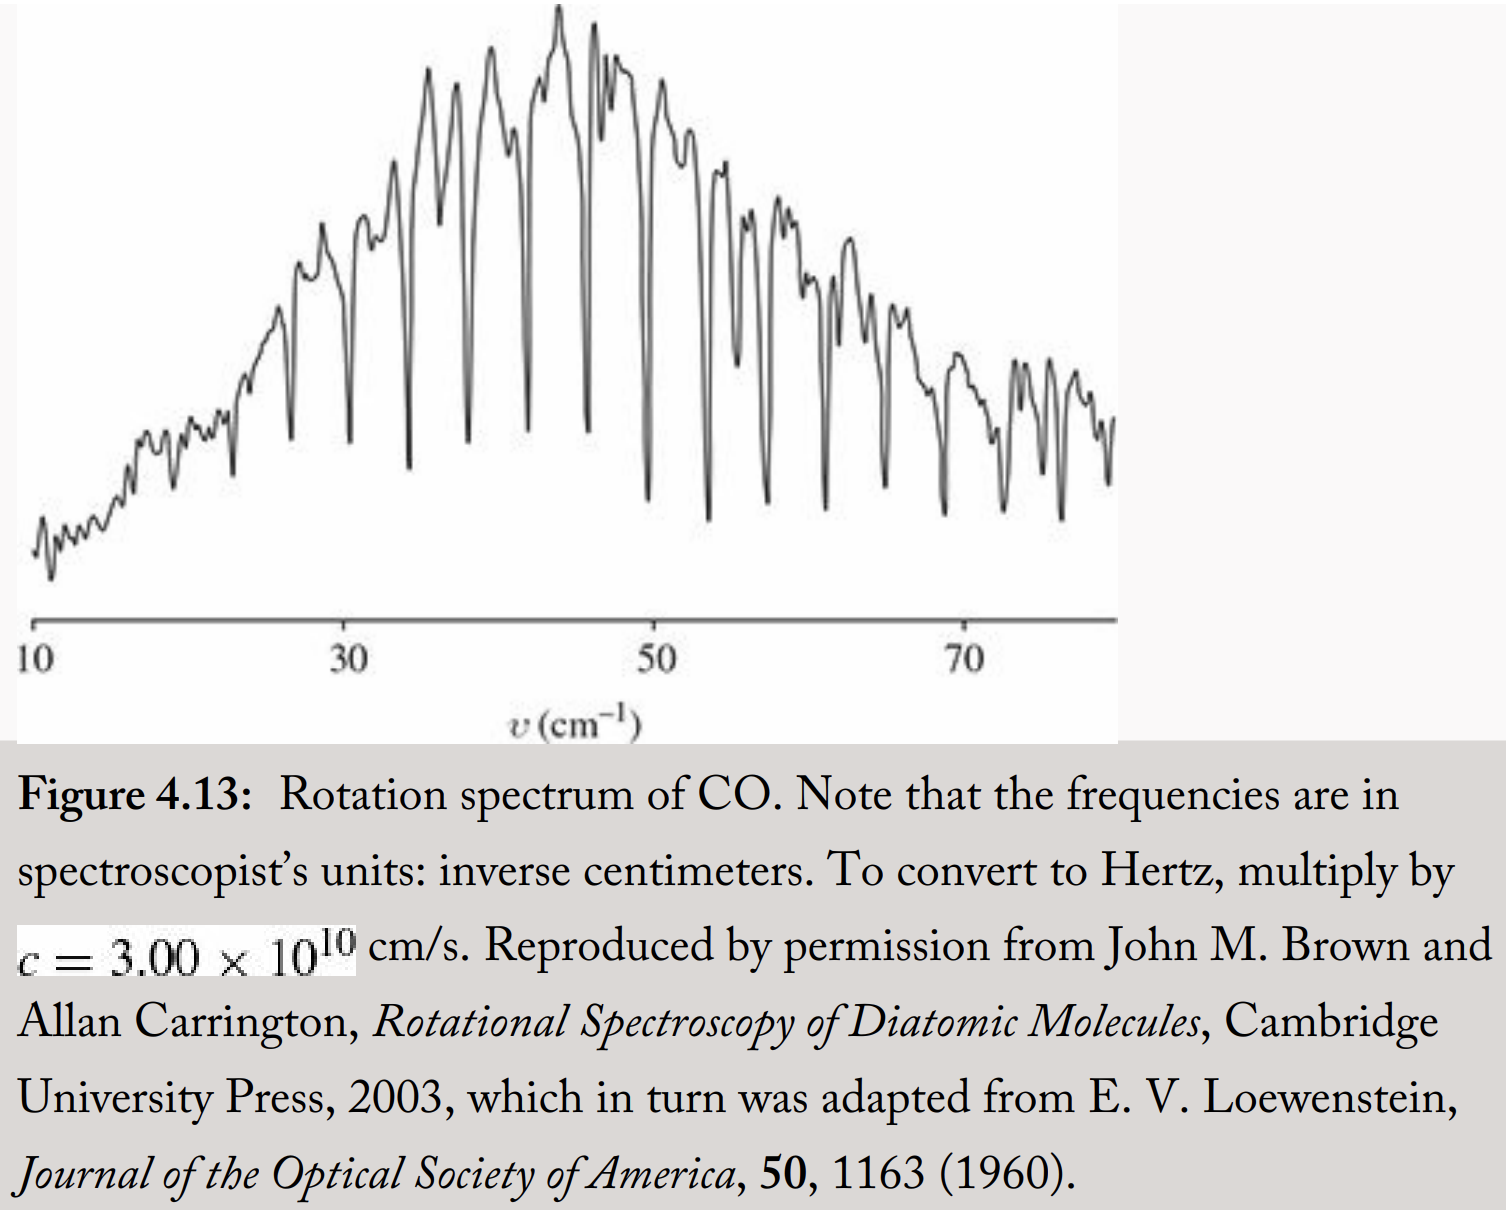
\includegraphics[width=100mm]{figure 4.13.png}
\end{itemize}
\end{ques}

\begin{proof}
    
\end{proof}

\newpage

\section*{5 ND}
\begin{ques}\label{q5}
Angular Ehrenfest

\begin{itemize}
\item[(a)] Prove the rotational analog to Ehrenfest’s theorem: for a particle in a general potential $V(r)$, the rate of change of the expectation value of the orbital angular momentum
$L$ is equal to the expectation value of the torque $\bN = \mathbf{r} \times (-\nabla V)$,
\[
\frac{d}{dt}\langle \bL \rangle = \langle \bN \rangle
\]

\item[(b)] Show that $d\langle \bL \rangle/dt = 0$ for any spherically symmetric potential. This is the quantum analog of the classical conservation of angular momentum
\end{itemize}
\end{ques}

\begin{proof}

    \hfil

    \begin{itemize}
        \item[(a)] First, using the classical definition, one gets the following:
        \begin{align}
            \bN &= \br \times (-\nabla V) \\
            &= -\left(y\frac{\partial V}{\partial z}-z\frac{\partial V}{\partial y}\right)\hat{x}-\left(z\frac{\partial V}{\partial x}-x\frac{\partial V}{\partial z}\right)\hat{y}-\left(x\frac{\partial V}{\partial y}-y\frac{\partial V}{\partial x}\right)\hat{z}
        \end{align}
        Now, assume one can directly promote each individual component to quantum-mechanical operators. Then, in the position basis, the expectation value of torque is givenn as follow:
        \begin{align}
            \left<\bN\right> &= -\left<y\frac{\partial V}{\partial z}-z\frac{\partial V}{\partial y}\right>\hat{x}-\left<z\frac{\partial V}{\partial x}-x\frac{\partial V}{\partial z}\right>\hat{y}-\left<x\frac{\partial V}{\partial y}-y\frac{\partial V}{\partial x}\right>\hat{z}
        \end{align}
        Now, using the definition $L_x = yp_z-zp_y$, the expectation value is given below (using the position basis, or the wave function):
        \begin{align}
            \left<L_x\right> = \int_{\RR^3}\psi^*(yp_z-zp_y)\psi dV
        \end{align}
        Which, incorporating the time derivative, assume the conditions are all satisfied (together with the position and momentum operators being time independent). Using the Schr\"odinger equation $\frac{\partial\psi}{\partial t} = \frac{(p_x^2+p_y^2+p_z^2)}{i\hbar 2m}\psi + \frac{V}{i\hbar}\psi$, together with the commutation relation $[u,p_v] = i\hbar\delta_{uv}, [p_u,p_v]=0, [u,v]=0$ for all $u,v \in \{x,y,z\}$ (which further implies$[u,p_u^2]=2i\hbar p_u$, and $[u,p_u^3] = 3i\hbar p_u^2$), one gets the following:
        \begin{align}
            \frac{d\left<L_x\right>}{dt} &= \frac{d}{dt}\int_{\RR^3}\psi^*(yp_z-zp_y)\psi dV = \int_{\RR^3}\left(\frac{\partial \psi}{\partial t}\right)^*(yp_z-zp_y)\psi + \psi^*(yp_z-zp_y)\frac{\partial\psi}{\partial t}dV
        \end{align}
    \end{itemize}
\end{proof}

\end{document}
